\documentclass{rapportENS}
\usepackage{lastpage}
\rfoot{\thepage  / \pageref{lastpage}}
\title{Title page}
\begin{document}

%----------- Informations du rapport ---------
\titre{Analyse de système mécatronique}
\Departement{Département Mécatronique}
\annee{$1^{ère}$ année}
\sujet{Rapport d'analyse de système mécatronique :\\ Ensemble Domotique EnOcean}
\enseignant{}
\eleves{Adrien \textsc{Vigné} - Martin \textsc{Filliung}}

%----------- Initialisation -------------------
\fairemarges{Vigné-Filliung} %Afficher les marges
\fairepagedegarde %Créer la page de garde
%\rfoot{\thepage  / \pageref{lastPage}}
\tabledematieres %Créer la table de matières

%------------ Corps du rapport ----------------

\part{Système étudié}
 \section{Présentation du système}
 La domotique à pour but d'interconnecter des sous-systèmes à la base indépendant afin d'améliorer l'interaction de l'ensemble avec son utilisateur. Ces technologies se retrouvent principalement dans l'habitat grâce à des capteurs connectés, des passerelle de contrôle ainsi que des actionneur ou des boîtiers de commande afin d'automatiser certaines actions ou de créer des alertes ou routine pour assister l'utilisateur. Ces installations demande d'être penser a la conception de la maison ou d'entreprendre des modifications afin de pouvoir les adapter à une installation existante car ils nécessitent entre autre une source d'énergie et ont un encombrement non négligeable. L'objet de cette étude à vocation à paliers à ces défauts en proposant une solution sans fils,sans alimentation externe et relativement peu encombrant afin de s'ajouter simplement à toute installation existante sans grande contraintes. 
 
 \section{Objectif du système}
 Cette ensemble domotique est l'ensemble proposé par la société \textit{EnOcean} avec des modules utilisant le principe de récupération d'énergie afin de minimiser leur impacts sur l'installation déjà présente. Le principe de récupération d'énergie est de permettre une indépendance énergétiques des modules au travers de transducteurs, tout en remplissant leurs objectifs d'interconnexion. Deux technologies employées pour répondre à ce critère seront étudié dans ce rapport.  Les fonctions principales du kit peut être représenter dans un diagrammes des interacteurs (Figure \ref{fig:Inter-acteurs}-\ref{tableau_cdcf})
 \begin{figure}[h!]
     \centering
     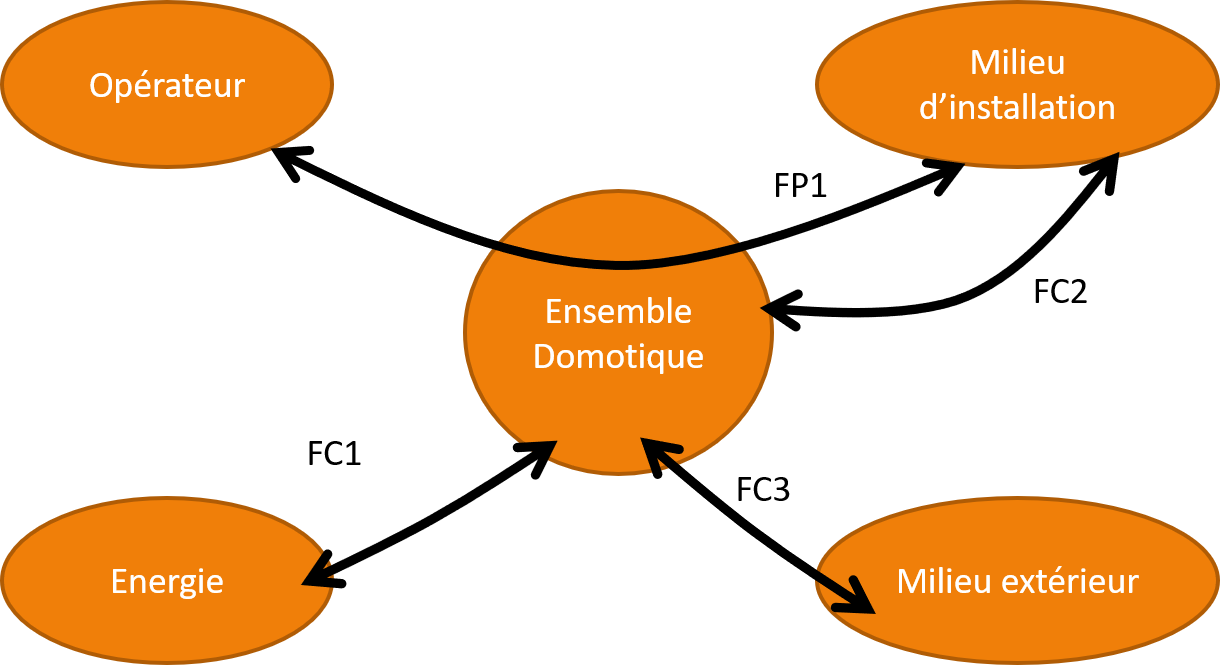
\includegraphics[width=0.9\linewidth]{Graphe_cdcdf.png}
     \caption{Diagramme des interacteurs}
     \label{fig:Inter-acteurs}
     \end{figure}
     \begin{figure}
         \centering
            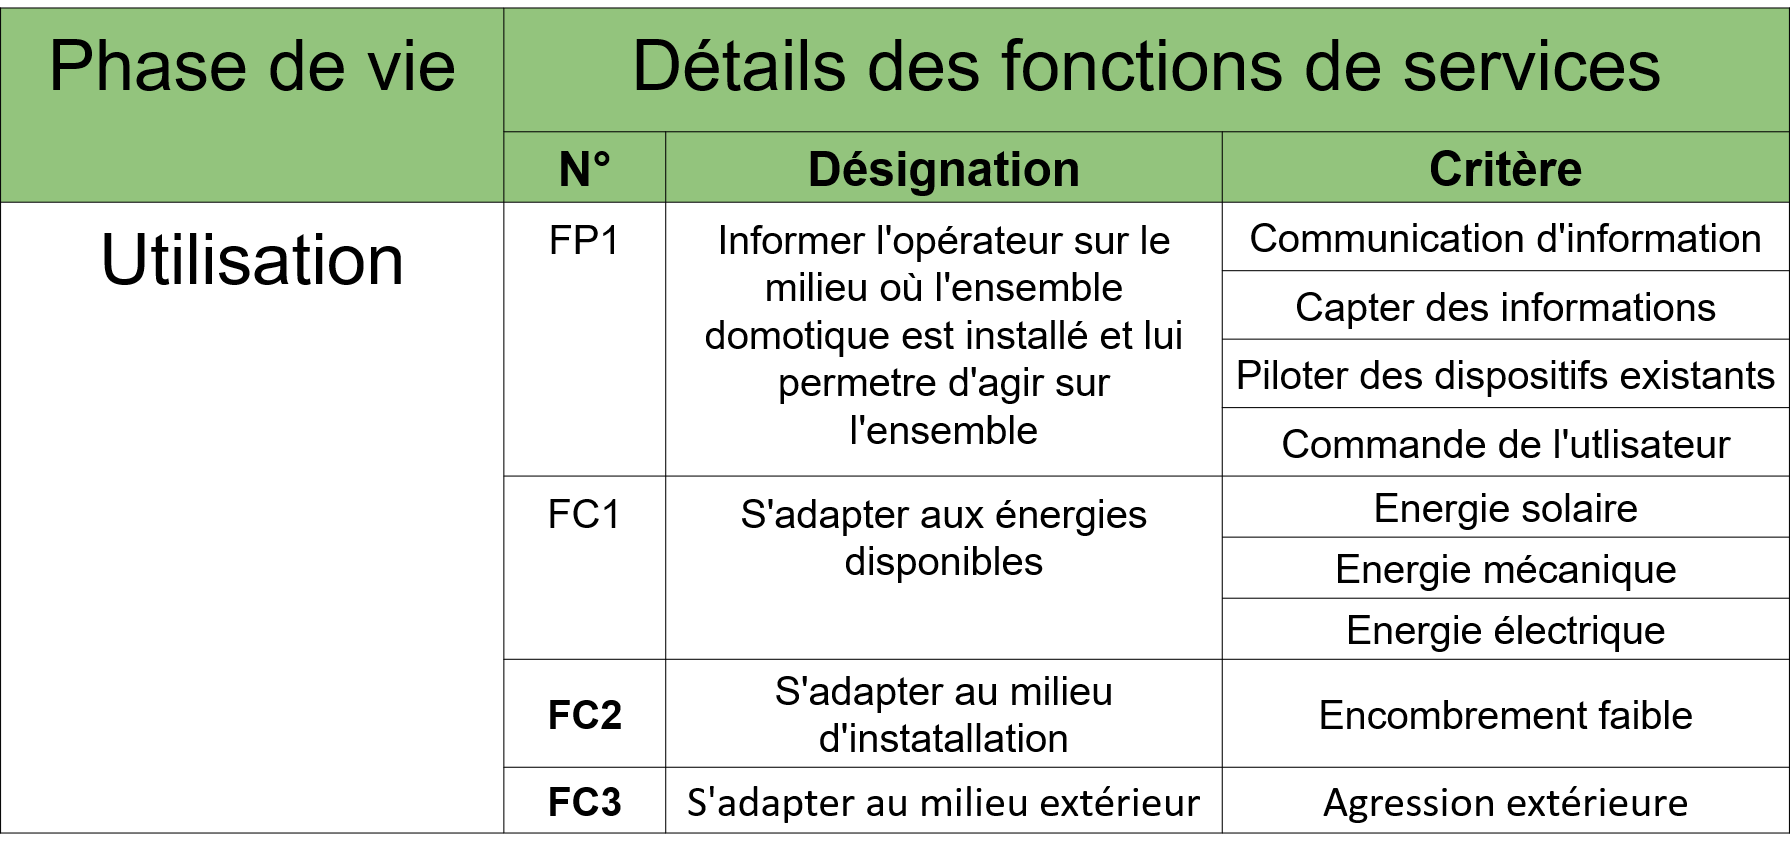
\includegraphics[width=\linewidth]{tableau_cdcf.png}
     \caption{Tableau du cahier des charges}
     \label{tableau_cdcf}
 \end{figure}


%  Cet ensemble de domotique a pour objectif de connecter et de rendre plus ergonomique l'utilisation de plusieurs systèmes propres à un logement : l'éclairage, le thermostat, sécurité, stores etc...
 
%  En connectant ces fonction à un poste centralisé relié à internet on peut diversifier les moyens de commande : interrupteur d'origine, interrupteur sans fils, smartphone, etc... pour l'éclairage. Cette diversité apporte le confort d'utilisation recherché. 

 \section{Caractéristiques du système}
 
 Les modules proposés par \textit{ubiwizz} sur très variés (Environ 180 articles listés). Mis a notre disposition sont :
 \begin{itemize}
 \item plusieurs interrupteurs sans piles 2 canaux;
 \item plusieurs capteurs de température et d'hydrométrie;
 \item un capteur d'ouverture de porte / fenêtre;
 \item un contacteur piloté;
 \item une passerelle \textit{EnOcean};
 \item un kit de développement;
 \item une passerelle programmable \textit{Raspberry Pi}. 
\end{itemize}  
 
 \section{Contraintes de conception}
 
 Les différents modules on pour contrainte d'être entièrement autonome une fois installés : ils ne doivent pas avoir à être rechargés, réinitialisés manuellement ou autrement manipulés pour bien fonctionner. De plus les modules doivent s'intégrer le plus facilement possible à l'environnement dans lequel on les place et donc être miniaturisés.
 
 \part{Étude du système}
 
 \section{Interrupteurs : alimentation sans pile}
 
 L'alimentation des interrupteurs sans fils est un circuit magnétique (aimant, fer et bobine, figure \ref{photocircuitmag}) dont la polarité de l'aimant peut être inversée grâce à une languette actionnée par l'utilisateur lorsqu'il presse le bouton (Figure \ref{schemacircuitmag}) il y a donc une partie mobile (en bleu et vert sur la figure \ref{schemacircuitmag} et une partie fixe dont l'aimant fait parti.
 
 \begin{figure}[h!]
 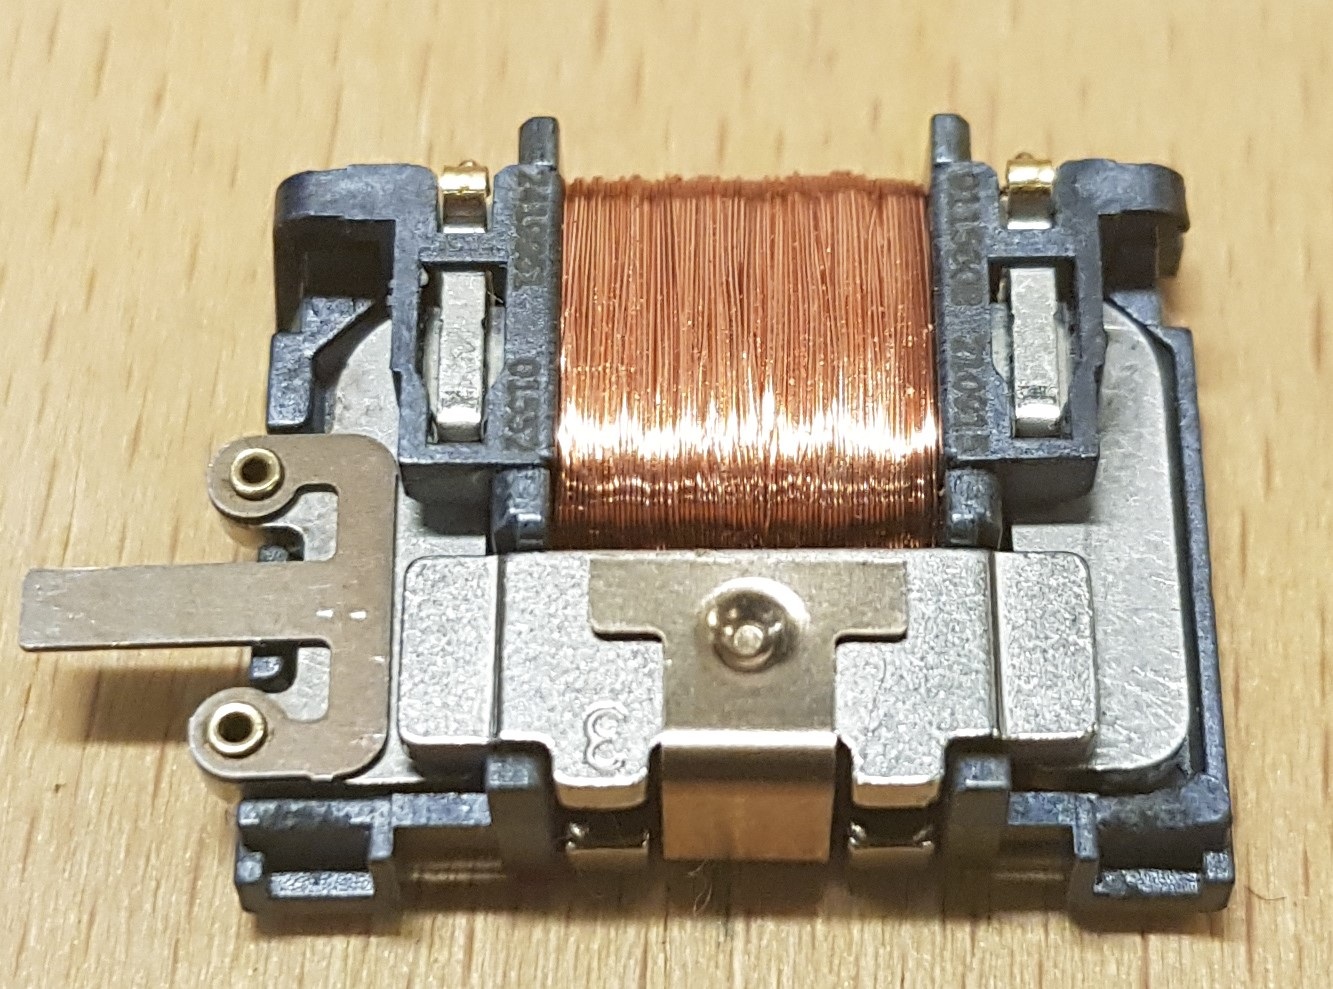
\includegraphics[width = .3\linewidth]{circuitmag.jpg}
 \centering
 \caption{Circuit magnétique alimentant les interrupteurs sans piles}
 \label{photocircuitmag}
 \end{figure}
 
 \begin{figure}[h!]
 \begin{subfigure}{.5\linewidth}
 \centering
 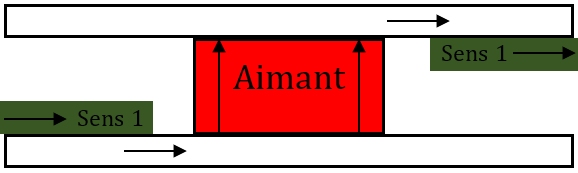
\includegraphics[width=.9\linewidth]{sens1.PNG}
 \caption{Sens 1 - direct}
 \label{sens1}
 \end{subfigure}
 \begin{subfigure}{.5\linewidth}
 \centering
 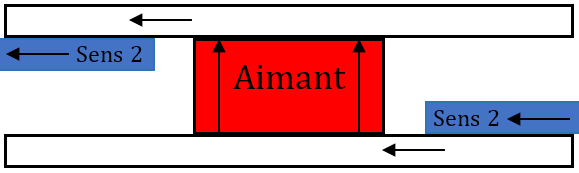
\includegraphics[width=.9\linewidth]{sens2.PNG}
 \caption{Sens 2 - inversé}
 \label{sens2}
 \end{subfigure}
 \caption{Différent positions du circuits magnétique}
 \label{schemacircuitmag}
 \end{figure}
 
 \subsection{Mesures et expériences}
 
 \subsubsection*{Mesure du pic de tension}
 
 
 
 \subsubsection*{Mesure du nombre de spires}
 
 Le nombre de spires est mesuré en faisant une seconde bobine sur le circuit magnétique dont on connais le nombre de spires $N_2 = 5$, le rapport des tensions $U_1$ et $U_2$ (figure \ref{nombredespire}) observés aux bornes des bobines sert a retrouver le nombre de spires $N_1$.
 
 \begin{figure}[h!]
  \centering
 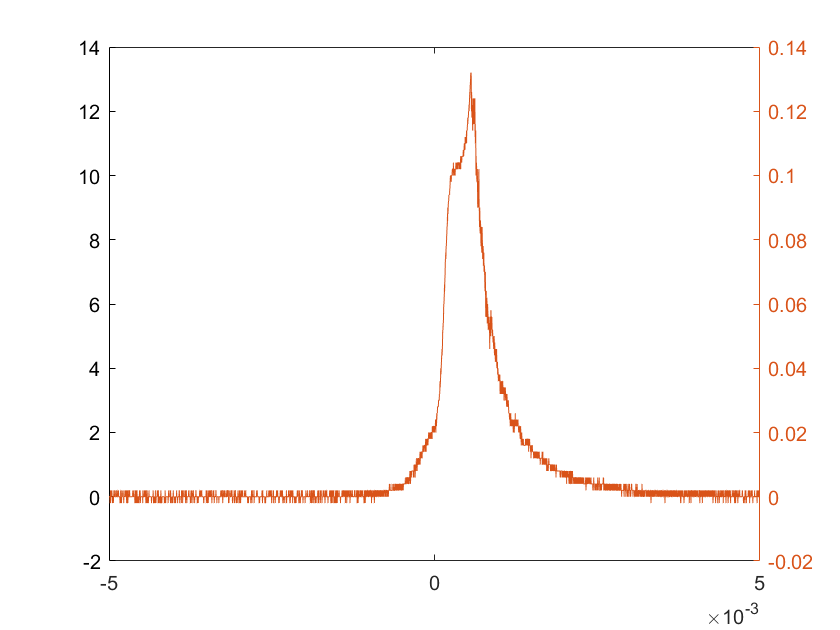
\includegraphics[width = .5\linewidth]{nombredespire.png}
 \caption{$U_1$ (axe de gauche) et $U_2$ (axe de droite) superposés}
 \label{nombredespire}
 \end{figure}
 
 \begin{equation}
     \frac{U_1}{U_2} = \frac{N_1}{N_2} \Leftrightarrow N_1 = \frac{U_1\cdot N_2}{U_2} = \frac{13V \times 5}{0,13V} = 500
 \end{equation}
 
 \subsubsection*{Mesure de l'entrefer maximum}
 
 Cette mesure est faire pour avoir une référence lors du calcul de l'entrefer $e$ avec la mesure de tension. On mesure d'abord le débattement $D$ dans la partie fixe puis l'épaisseur $E$ de la partie mobile.
 
 \begin{equation}
     e_{max} = \frac{D-E}{2} = 1,5\times 10^{-4} m
 \end{equation}
 
 \subsection{Étude théorique}
 
 Lorsqu'on actionne l'interrupteur on observe un bref pic de tension aux bornes de la bobine (mesure faite à l'osciloscope, figure \ref{tensionobine}).
 
 \begin{figure}[h!]
 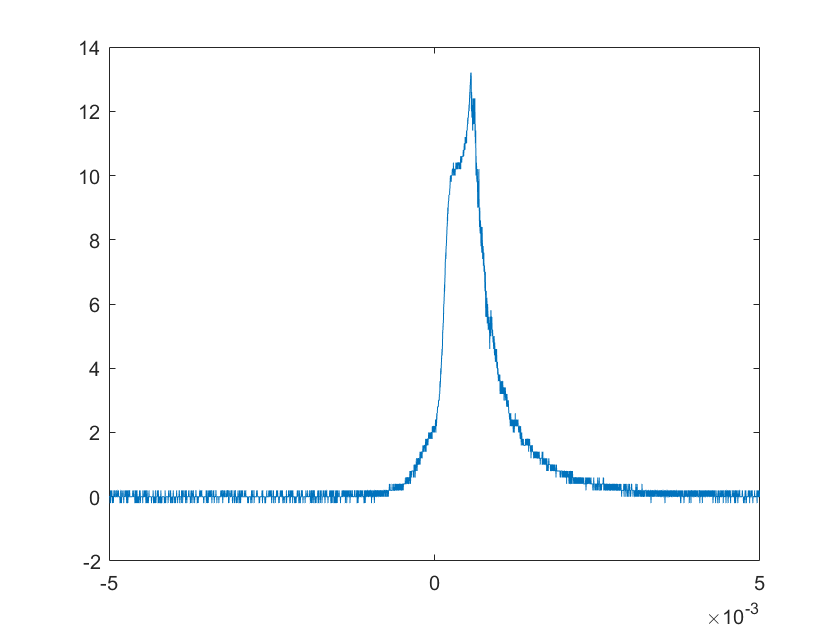
\includegraphics[width = .5\linewidth]{tension.png}
 \centering
 \caption{Tension ($Volts$) en fonction du temps ($secondes$)}
 \label{tensionobine}
 \end{figure}
 
 Avec ces données on peut directement obtenir le flux total \textit{"vu"} par la bobine avec la Loi de Lenz (Figure \ref{fluxobine}):
 
 \begin{equation}
 \Phi_{tot}(t) = -\int U(t) dt
 \end{equation}
 
 \begin{figure}[h!]
 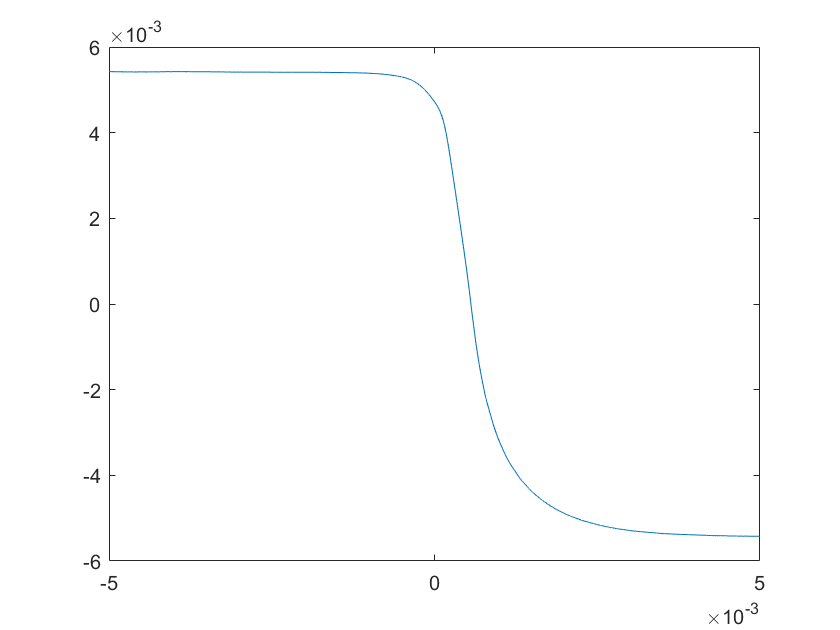
\includegraphics[width = .5\linewidth]{flux.png}
 \centering
 \caption{Flux ($Wb$) en fonction du temps ($secondes$)}
 \label{fluxobine}
 \end{figure}
 
 Puis avec la définition du flux magnétique on obtient le champ magnétique (Figure \ref{champ}): 
 
 \begin{equation}
 \Vert \overrightarrow{B}(t) \Vert = \frac{\Phi_{tot}(t)}{N \cdot dS}
 \end{equation}
 
 \begin{figure}[h!]
 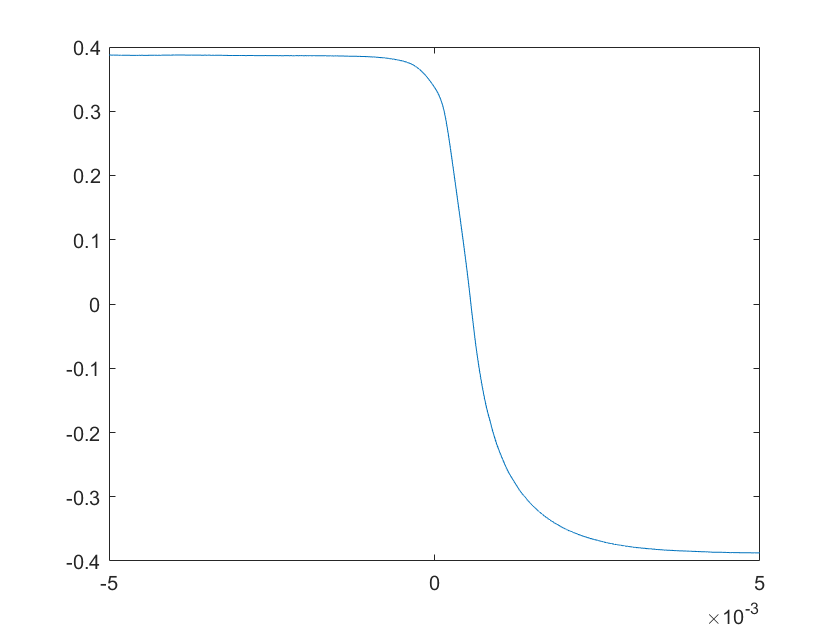
\includegraphics[width = .5\linewidth]{champmag.png}
 \centering
 \caption{Champ magnétique ($T$) en fonction du temps ($secondes$)}
 \label{champ}
 \end{figure}
 
 Avec $N$ le nombre de spire dans la bobine obtenue avec le protocole suivant :
 
On enroule un nombre connu de spires sur le circuit magnétique puis on actionne l'interrupteur en relevant les pics de tension aux bornes des deux enroulements. On déduis le nombre de spires avec le rapport des valeurs des pics et le nombre de spires du second enroulement.

On peut en suite déduire l'entrefer en supposant que la perméabilité du fer est très grande devant celle du vide et donc négligeable :

 \begin{equation}
 e(t) = \frac{\mu_0 \cdot dS}{\Phi_{tot}(t)}
 \end{equation}
 
 \section{Caractérisation du panneau solaire}
 
 \part{Conclusion}
 
 \part{Bibliographie}
\end{document}